\documentclass[12pt,a4paper]{article}
\usepackage{setspace}   % paquete para interlineado
\usepackage{newtxtext,newtxmath} % Times New Roman

%haber si funciona mas parecido a word
\setstretch{1.5}  
%\usepackage[protrusion,expansion]{microtype}
%\onehalfspacing               % interlineado 1.5
\usepackage{amsmath} % Para usar \text{}
\usepackage[utf8]{inputenc}
\usepackage[spanish]{babel}
\usepackage[left=3cm, right=2.5cm, top=2.5cm, bottom=2.5cm]{geometry}
\usepackage{graphicx}
\usepackage{titlesec}
\usepackage{setspace}
\usepackage{lipsum}
\geometry{margin=1in}



 % PAQUETE PARA INSTANCIAR  LAS IMAGENES
  \graphicspath{{./Imagenes}}
 

%CONFIGURACION DE MI PAGINA numeración:
\usepackage{fancyhdr}
\pagestyle{fancy}
\fancyhf{} % Limpia encabezados/pies
\fancyhead[R]{\thepage} % Números arábigos arriba: izq en pares, der en impares
\renewcommand{\headrulewidth}{0pt} % Sin línea

%COLOCAR NUMERACION ESQUINA DERECHA PAG 1
\fancypagestyle{plain}{%
	\fancyhf{}%
	\fancyhead[R]{\thepage}%
	\renewcommand{\headrulewidth}{0pt}%
}


% --- PAQUETES ADICIONALES DE LOSA ---
  % para listas multinivel (numeración + incisos + viñetas)
\usepackage{enumitem} 
% que los párrafos  de las secciones dentro de los items usen la misma sangría que el cuerpo SANGRIA A TODOWWW
\setlist[enumerate]{listparindent=\parindent, parsep=0pt}



% --- Configuración de enumitem para numeración multinivel ---
\setlist[enumerate,1]{label=\arabic*., leftmargin=1.2cm}
\setlist[enumerate,2]{label=\arabic{enumi}.\arabic*., leftmargin=1.4cm}
\setlist[enumerate,3]{label=\arabic{enumi}.\arabic{enumii}.\arabic*., leftmargin=1.6cm}
\setlist[enumerate,4]{label=\alph*) , leftmargin=1.8cm}
\setlist[itemize]{leftmargin=1.6cm}




\begin{document}
	\thispagestyle{fancy} 
	
	\titleformat{\section}{\large\bfseries}{\thesection.}{0.5em}{}
	\titleformat{\subsection}{\normalsize\bfseries}{\thesubsection.}{0.5em}{}
	
	\title{\vspace{-2cm}Área de Métodos Constructivos
	\\ Descripción y proceso constructivo de losas}
	\author{}
	\date{}
	
	
	
	
	
	
	\maketitle
	
	\vspace{-2.5cm}
	
	
	
	
	
	
	
	
	
%-------------LOSA TRADICIONAAAAL--------------------




	\section{Losa Tradicional}

La losa tradicional, también llamada losa maciza, es un elemento estructural sólido de concreto reforzado, soportado por vigas o muros, con espesor uniforme en toda su extensión. Se utiliza de manera frecuente en edificios residenciales, comerciales e industriales, así como en obras donde se presentan cargas concentradas importantes que requieren alta rigidez y continuidad estructural.

El proceso constructivo de este tipo de losa constituye una de las actividades más relevantes dentro de la ejecución de estructuras de concreto en Guatemala. Su correcta ejecución no solo depende de la experiencia de la mano de obra, sino también del cumplimiento de normas y códigos técnicos que establecen criterios de diseño, recubrimientos, tolerancias y tiempos adecuados de curado y desencofrado. Entre ellos destacan la Norma Sísmica de Edificación NSE 7.1 (que adopta el ACI 318S-19), la guía ACI 347R para encofrados y la ACI 308R sobre curado del concreto, además de normas guatemaltecas como la NTG 41068 para concreto premezclado.

En este sentido, el proceso constructivo de una losa tradicional maciza incluye fases claramente definidas: preparación del sitio, montaje del encofrado y apuntalamiento,  del acero de refuerzo, vaciado del concreto, curado y desencofrado. El cumplimiento ordenado y riguroso de cada etapa asegura que la losa alcance la resistencia, durabilidad y seguridad estructural necesarias, garantizando su adecuado desempeño como diafragma rígido y elemento portante dentro de la edificación.

%\vspace{0.5} % agrega 1 cm de espacio
\begin{figure}[h]
	\centering
	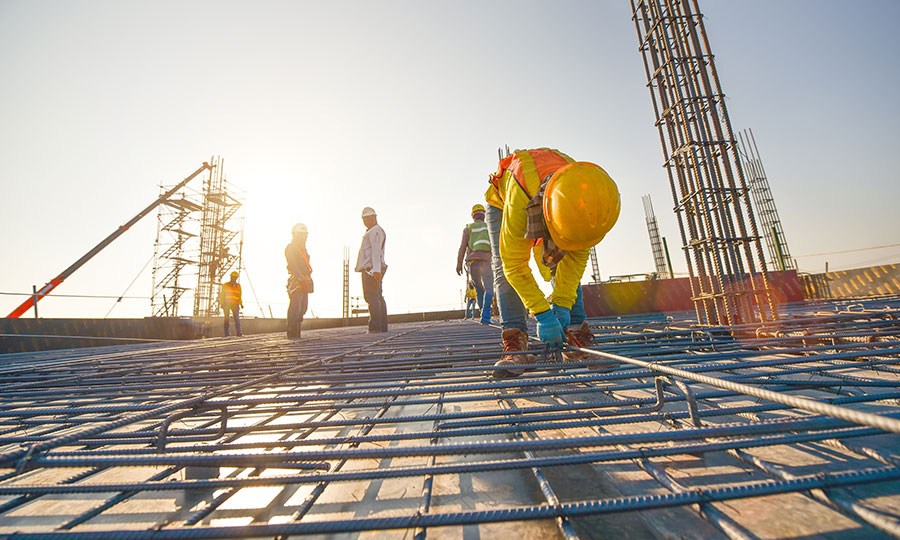
\includegraphics[width=0.6\textwidth]{losa1}
	\caption{Proceso de armado con retícula y refuerzos perimetrales}
	\label{fig:losa1}
\end{figure}

	\subsection{Preparación y limpieza del sitio}
	Se debe tener un ambiente de trabajo limpio y libre de obstáculos, en el que se
	puedan movilizar libremente las personas y maquinarias que participarán en la
	obra. Este paso incluye la deforestación y remoción de cualquier capa vegetal que
	pudiera entorpecer el trabajo, la limpieza y explanación del terreno en caso de
	tratarse de una losa de fundación o la losa de la planta baja. Procesos a considerar:
	\begin{enumerate}
		\item Retirar escombros, basura y obstáculos del área de trabajo.
		\item Nivelar y trazar el perímetro conforme a planos estructurales.
		\item Preparar accesos para el traslado de materiales y equipos.
	\end{enumerate}
	
	%\vspace{0.5} % agrega 1 cm de espacio
	\begin{figure}[h]
		\centering
		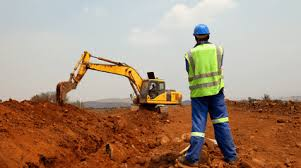
\includegraphics[width=0.6\textwidth]{losa2}
			\caption{Limpieza de terreno}
		\label{fig:losa2}
	\end{figure}
	
	%-----------------------------
	
	\subsection{Preparación de Materiales y herramientas}
	Al momento de iniciarse la obra se deben contar con todos los implementos que
	se van a necesitar al igual que tener todos los materiales a disposición para que el
	proceso no se vea interrumpido o paralizado por la falta de alguno de los
	anteriores.
	
	Como se observa en la figura 3, se encuentran elementos como materiales, maquinarias y herramientas
	necesarias para la jornada planificada. En el fondo la arena y la piedra picada, a la
	derecha las cabillas y la malla electrosoldada. Puntales de acero, madera para
	encofrado, mezcladora de concreto, etc.
	
	
	
	\begin{enumerate}
		\item \textbf{Herramientas}
		\begin{enumerate}[label=\alph*)]
			\item Serrucho, martillo, escuadra, plomada, nivel, cinta métrica.
			\item Palas, picos, carretillas y regletas metálicas.
			\item Ganchos para amarre y dobladora de varilla.
		\end{enumerate}
		\item \textbf{Equipos}
		\begin{enumerate}[label=\alph*)]
			\item Mezcladora, vibrador de aguja, andamios y escaleras.
			\item Sistemas de izaje o bombas de concreto en niveles superiores.
		\end{enumerate}
		\item \textbf{Materiales}
		\begin{enumerate}[label=\alph*)]
			\item Cemento Portland, arena, grava y agua potable.
			\item Acero de refuerzo y malla electrosoldada.
			\item Tuberías PVC para instalaciones eléctricas e hidrosanitarias.
			\item Madera o formaletas metálicas y desmoldante.
		\end{enumerate}
	\end{enumerate}
	
	\begin{figure}[h!]
		\centering
		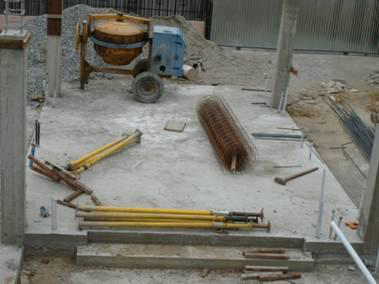
\includegraphics[width=0.6\textwidth]{losa3}
		\caption{Materiales y herramientas}
		\label{fig:losa3}
	\end{figure}
	
	%---------------------------------
	
	
	\subsection{Encofrado y apuntalamiento}

	El encofrado es la \textit{estructura temporal} que da forma al concreto fresco, soporta su peso y mantiene en posición el refuerzo hasta que la mezcla alcance resistencia.
	
	Su función principal es ofrecer la posibilidad de que el acero de refuerzo
	sea colocado en el sitio correcto, darle al concreto la forma y servirle de apoyo
	hasta que endurezca, está constituido por el molde y los puntales, que pueden ser
	metálicos o de madera. Existen una gran cantidad de tipos de encofrado, de distintos materiales y de
	distintas formas, cada uno es utilizado para un fin específico
	
	\subsubsection{Tipos de encofrado}
	
	\begin{enumerate}
		\item \textbf{Madera}
		
		Presentan la ventaja de que pueden ser cortados para
		darles la forma deseada, sin embargo esto genera desperdicios de material que en
		ocasiones no se puede reutilizar. Para alargar la vida útil del encofrado y que se
		pueda reutilizar en distintas obras se le debe dar un cuidado especial como se
		indica:
		
		\begin{enumerate}[label=\alph*)]
			\item Fácil de cortar y adaptar a diferentes geometrías.
			\item Debe limpiarse y almacenarse protegido para prolongar su vida útil.
			\item Aplicar desmoldante para facilitar el desencofrado.
		\end{enumerate}
		\item \textbf{Metálico}
	
		Los encofrados metálicos presentan un desgaste mínimo con un manejo
		adecuado. Al igual que los de madera deben ser tratados de manera especial:
		
		
		\begin{enumerate}[label=\alph*)]
			\item 
			Se deben limpiar bien luego de usarlos, e impregnarlos con un producto
			desmoldante comercial: aceite, petróleo o gasoil con parafina al 50%,
			dependiendo del acabado que se quiera lograr.
			\item 
			Se debe evitar la oxidación protegiéndolos periódicamente con pintura
			anticorrosiva, sobre todo si van a estar mucho tiempo a la intemperie.
			
			\item 
			Debe protegérsele también de los rayos del sol y de la lluvia.
			
			\item 
			Se debe almacenar en sitios cubiertos y secos, debidamente codificados,
			colocado verticalmente o ligeramente inclinado cuando se recuesten sobre
			un muro y levantados del piso sobre zancos o tacos.
			
		\end{enumerate}
		
		
		\item \textbf{Plástico (casetones)}
		
		Son los más usados para el vaciado de losas nervadas y
		reticulares ya que vienen con formas y dimensiones predefinidas para tal fin. Su
		principal ventaja es que son muy fáciles de manipular y colocar en sitio debido a
		su ligereza
		
		\begin{enumerate}[label=\alph*)]
			\item Usados en losas nervadas o reticulares.
			\item Ligeros y de fácil manipulación, aunque delicados.
		\end{enumerate}
	\end{enumerate}
	
	
	\begin{figure}[h]
		\centering
		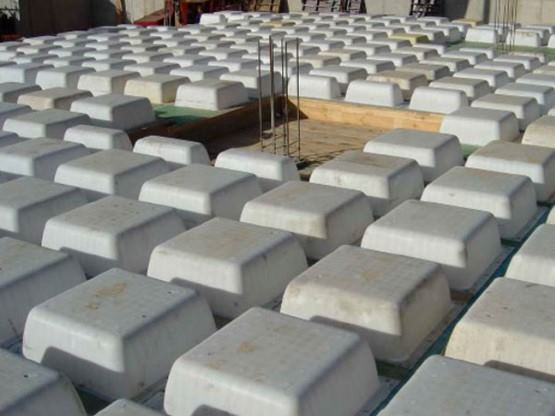
\includegraphics[width=0.7\textwidth]{losa4}
		\caption{Sistema de casetones recuperable}
		\label{fig:losa4}
	\end{figure}
	
	
	
	\subsubsection{Puntales}
	
	Los puntales los elementos que le proporcionan soporte al encofrado hasta
	que el concreto fragüe y la estructura sea capaz de resistir las cargas debidas a su
	propio peso
	
	\begin{enumerate}
		\item Los puntales pueden ser de madera o metálicos telescópicos.
		\item Deben colocarse plomados, sobre bases firmes y arriostrados.
		\item Su función es resistir el peso del concreto fresco y cargas de construcción.
	\end{enumerate}
	

	\begin{figure}[h]
	\centering
	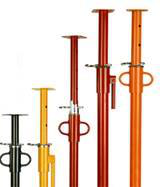
\includegraphics[width=0.35\textwidth]{losa5}
	\caption{Puntales Metálicos}
	\label{fig:losa5}
\end{figure}

	
	\subsection{Colocación del acero de refuerzo Inferior}
	Luego de haber encofrado y apuntalado correctamente la losa se procede a la
	colocación del acero de refuerzo de la misma. Es evidente que previamente se
	debió haber cortado y doblado las cabillas de acuerdo a los planos del despiece.
	Es importante que las barras se fijen firmemente en su posición para evitar que se
	muevan cuando se esté vaciando el concreto, también debemos respetar los
	recubrimientos que deben tener, si es necesario se pueden apoyar sobre tacos de
	concreto que tengan una altura igual a la del recubrimiento y una resistencia
	mayor o igual a la del concreto que se vaciará en la losa.
	
	
	\subsection{Colocación de las tuberías y conductos para
		instalaciones eléctricas e hidrosanitarias}
		
		De acuerdo al uso de la edificación o del nivel que se esté por construir, se puede
		decidir entre embutir las tuberías y conductos en la losa o si colgarlos para que
		vayan debajo de la misma, quedando a la vista desde el nivel inferior. De cualquier
		manera se deben ubicar en su posición antes de vaciar el concreto. En el caso de
		las tuberías destinadas a las instalaciones eléctricas se recomienda pintarlas o
		etiquetarlas de manera que se puedan distinguir entre las tuberías de apagadores,
		tomacorrientes, etc.
		
	\begin{enumerate}
		\item Instalar tuberías eléctricas e hidrosanitarias antes del vaciado.
		\item Sujetar firmemente para impedir movimiento.
		\item Etiquetar tuberías eléctricas para identificación.
	\end{enumerate}
	
	\subsection{Colocación del acero de refuerzo superior}
	Se coloca el acero superior teniendo las mismas precauciones que el acero
	inferior. Si no se requiere de la colocación de barras de refuerzo se coloca la malla
	electrosoldada de acuerdo a los planos de despiece.
	
	\begin{enumerate}
		\item Colocar varillas o malla electrosoldada en la parte superior.
		\item Respetar los recubrimientos mínimos.
	\end{enumerate}
	
	\begin{figure}[h]
		\centering
	%	\includegraphics[width=0.7\textwidth]{armado.jpg}
		\caption{Armadura y malla electrosoldada en losa.}
	\end{figure}
	
	\subsection{Vaciado del concreto}
	Luego de tener todos los elementos de la losa ubicados en su sitio, se lleva a cabo
	el proceso de vaciado de concreto, el cual puede ser mezclado en obra o traído de
	una planta de premezclado.
	El vaciado se puede realizar con la utilización de herramientas simples como
	baldes y carretillas si se trata de la planta baja o los niveles inferiores de la
	edificación (máximo hasta el segundo nivel) con la ayuda de un sistema de poleas.
	Para niveles superiores se puede realizar con la utilización de una grúa y un
	carretón, o mediante la utilización de bombas que lleven el concreto a través de
	tuberías.
	
	\subsubsection{Procedimiento}
	\begin{enumerate}
		\item Transportar el concreto en carretillas, baldes o mediante bomba.
		\item Descargar en capas uniformes para evitar segregación.
		\item Vibrar con aguja para compactar y eliminar vacíos.
		\item Nivelar con reglas metálicas y palustre.
	\end{enumerate}
	
	\begin{figure}[h]
		\centering
	%	\includegraphics[width=0.7\textwidth]{vaciado.jpg}
		\caption{Proceso de vaciado del concreto en losa.}
	\end{figure}
	
	\subsection{Curado de concreto}
	El objetivo principal del curado es el de evitar que se evapore el agua de la
	mezcla, lo que podría producir grietas de retracción debido a la pérdida de
	humedad y alteraciones en la relación agua/cemento de la mezcla, lo que incide
	directamente en su resistencia. Para obtener mejores resultados, se recomienda
	humedecer el concreto durante los primeros 7 días de vaciado.
	El proceso del curado empieza incluso antes del vaciado del concreto, al mantener
	humectado el encofrado, para así evitar la pérdida del agua por la absorción de la
	madera.
	
	\subsubsection{Métodos}
	\begin{enumerate}
		\item Mantener la superficie húmeda al menos durante 7 días.
		\item Aplicar riego frecuente o cubrir con plásticos/membranas.
		\item En climas cálidos: regar más seguido y proteger con sacos mojados.
		\item En climas fríos: prolongar el curado por el fraguado lento.
	\end{enumerate}
	
	\begin{figure}[h]
		\centering
	%	\includegraphics[width=0.7\textwidth]{curado.jpg}
		\caption{Curado superficial de losa maciza.}
	\end{figure}
	
	\subsection{Desencofrado y desapuntalamiento}
	Una vez iniciado el fraguado del concreto se pueden comenzar a retirar los
	encofrados laterales de la losa y posteriormente se pueden retirar algunos
	puntales. El desapuntalamiento se debe ir haciendo en forma progresiva a medida
	que van pasando los días, hasta que se pueden retirar todos los puntales y el
	encofrado a los 21 días.
	
	\subsubsection{Criterios}
	\begin{enumerate}
		\item Retirar primero las formaletas laterales.
	%	\item Quitar los puntales en forma progresiva tras alcanzar la resistencia mínima (≈70\% f’c).
		\item Completar el desapuntalamiento a los 21 días, salvo indicación distinta en planos.
	\end{enumerate}
	
	\begin{figure}[h]
		\centering
	%	\includegraphics[width=0.7\textwidth]{desencofrado.jpg}
		\caption{Proceso de desencofrado y retiro de puntales.}
	\end{figure}
	
	%---------------LOSA NERVADA--------------------
	
	\section{Descripción y proceso constructivo de Losa Nervada}
	
	La losa nervada es un elemento de concreto reforzado compuesto por una losa de compresión delgada apoyada sobre nervios (viguetas) de concreto (con o sin casetones/aligerantes). Se usa para cubrir luces medianas reduciendo peso propio respecto a losas macizas. En Guatemala, el diseño de concreto estructural se rige por \textbf{NSE 7.1 (AGIES)}, que armoniza con \textbf{ACI 318}; tolerancias y aspectos constructivos también se alinean con \textbf{ACI 117} y \textbf{ACI 301}.
	
	\subsection{Normas de referencia}
	\begin{itemize}
		\item \textbf{Guatemala – AGIES / NSE 7.1 (2018)}: norma base para concreto estructural en edificaciones (criterios de diseño, cuantías, recubrimientos, detallado, tolerancias de construcción).
		\item \textbf{ACI 318 (ed. vigente en proyecto)}: requisitos de diseño/armado para losas (incluye sistemas de \textit{one-way joist} y \textit{two-way waffle}), límites de deflexión, recubrimientos, anclajes.
		\item \textbf{ACI 347 / 347R (Guide to Formwork for Concrete)}: encofrados (diseño, presiones de colado, apuntalamiento, secuencias y seguridad).
		\item \textbf{ACI 308R (Guide to Curing Concrete)} y ACI 308.1: curado externo (métodos y tiempos recomendados por desempeño/ambiente).
		\item \textbf{ACI 117}: tolerancias de construcción. Estas se integran también en la \textbf{NSE 7.1}.
	\end{itemize}
	

	
	\subsection{ Encofrado y Apuntalamiento}
	\begin{enumerate}
		\item \textbf{Trazado y replanteo} de ejes, espesores, modulación de nervios y huecos/casetones según planos. Coordinar con pasos de instalaciones (electroductos, desagües).
		\item \textbf{Vigas/muros de borde}: verificar cotas de apoyo y niveles.
		\item \textbf{Montaje de encofrado}: 
		\begin{itemize}
			\item Fondo de losa (tableros/terciado/metálico) con apuntalamiento que controle flechas inmediatas de la cimbra; usar aceite desmoldante compatible.
			\item Moldes de nervios/casetones: colocar, alinear y amarrar para evitar flotación o movimiento durante el colado; prever pases para vibrador.
			\item Rigidez y estanqueidad: evitar pérdidas de mortero y rotaciones locales; ACI 347/347R enfatiza continuidad, estabilidad, y control de deformación de la cimbra.
		\end{itemize}
		\item \textbf{Revisiones previas (checklist)}: niveles, flechas admisibles de cimbra, verticalidad, diámetros de pernos, separación de puntales, accesos y seguridad (barandas, andamios), certificaciones de la cimbra metálica si aplica. (ACI 347/347R).
	\end{enumerate}
	
	\subsection{ Armado (Refuerzo)}
	\begin{enumerate}
		\item Colocación de acero de nervios (longitudinal + estribos/amilletado si especificado) y malla o barras en la losa de compresión; respeta recubrimientos y empalmes según NSE 7.1/ACI 318.
		\item Uso de distanciadores (calzos) para asegurar recubrimiento; controla que los casetones no lo reduzcan.
		\item Detalle en apoyos: negativos sobre vigas, ganchos, anclajes; continuidad en juntas frías planificadas.
		\item Pasos de instalaciones: deja embebidos/tuberías según planos para no cortar nervios o acero principal.
		\item Control dimensional: NSE 7.1 incluye figuras de tolerancias constructivas basadas en ACI 117; respétalas para evitar no conformidades.
	\end{enumerate}
	
	\subsubsection{Vaciado (Instalación del Concreto)}
	\begin{enumerate}
		\item Revisar la cimbra justo antes: limpieza, humedad superficial (no encharcada), desmoldante uniforme.
		\item Concreto: asentamiento (slump) y tamaño máximo de agregado acordes a congestión de acero y geometría de nervios; programa de control de calidad (muestreo para f’c).
		\item Secuencia de colado: llenar uniformemente los nervios y luego la losa de compresión, evitando empujes desequilibrados que roten la cimbra. ACI 347 da pautas para secuenciación y control de presión.
		\item Vibrado interno (en nervios) + regla/llana en capa de compresión; cuida no desplazar casetones ni acero.
		\item Acabado: nivelación final y textura requerida (broom/llaneado) según uso.
	\end{enumerate}
	
	\subsubsection{ Curado}
	\begin{itemize}
		\item Iniciar tan pronto como la superficie lo permita para evitar pérdida temprana de humedad. Métodos: compuestos de curado, mantas húmedas, láminas impermeables (polietileno), o curado con agua; elegir según clima/uso. ACI 308R reúne procedimientos, tiempos orientativos y compatibilidades con acabados.
		\item Duración: mantener humedad/temperatura suficientes hasta alcanzar desempeño (p. ej., $\geq$7 días en clima templado o hasta lograr \% de f’c requerido para desencofrado/carga). Referencias técnicas de pavimentos y ACI 308 orientan duraciones y tasas de aplicación de compuestos.
	\end{itemize}
	
	\subsubsection{ Desencofrado y Retiro de Puntales}
	\begin{itemize}
		\item No retirar antes de cumplir la resistencia mínima especificada por el ingeniero (p. ej., \% de f’c o días) y verificación de flechas; ACI 347/347R da criterios para desencofrado gradual y reapuntalamiento en losas continuas.
		\item Inspección posterior: revisar nidos de grava, panza en nervios, fisuras tempranas, nivelaciones.
	\end{itemize}
	
	\subsection{Ventajas y Desventajas}
	
	\subsubsection{Ventajas}
	\begin{itemize}
		\item Menor peso propio que losa maciza $\rightarrow$ alta eficiencia para luces medianas, menor demanda sísmica y en elementos soportantes (Aplica con criterios AGIES/ACI).
		\item Posibilidad de prefabricar o usar encofrado repetible (casetones/panes), agilizando rendimientos.
		\item Aprovecha rigidez direccional (one-way joist) o bidireccional (waffle), optimizando materiales según arquitectura.
	\end{itemize}
	
	\subsubsection{Desventajas}
	\begin{itemize}
		\item Mayor complejidad de encofrado (más piezas, mayor control de alineación, riesgo de flotación de casetones).
		\item Coordinación más estricta con instalaciones para no interferir con nervios.
		\item Acabado inferior expuesto: si queda a la vista, exige mejor acabado de cimbra o revestimiento posterior (costo).
		\item Dependencia de control de curado y tiempos de cimbra para evitar fisuras/excesos de flecha temprana.
	\end{itemize}
	
	\subsection{Buenas Prácticas y Recomendaciones Normativas}
	\begin{itemize}
		\item Antes de colar: checklist de cimbra (rigidez, flecha admisible, nivel), recubrimientos medidos, limpieza, y prueba piloto de vibrado en un tramo (ACI 347/347R).
		\item Diseño por servicio: verificar deflexiones y espesores mínimos de capa de compresión según ACI 318; si no cumples límites simplificados, calcular flechas inmediatas + diferidas.
		\item Curado: seleccionar método acorde a clima de obra (altitud / vientos en Xela) y uso final; documentar tasa y frecuencia (ACI 308R/308.1).
		\item Tolerancias: aplicar las figuras y comentarios de tolerancias de la NSE 7.1 (basado en ACI 117) para ubicación de acero, niveles y espesores.
	\end{itemize}
	
	\subsection{Resumen del proceso de construcción}
	\begin{enumerate}
		\item Cimbrar + apuntalar + casetones.
		\item Colocar acero (nervios + losa) y separadores.
		\item Revisiones y pre-colado.
		\item Colado por tramos con vibrado en nervios.
		\item Acabado de losa.
		\item Curado continuo ($\geq$7 días o hasta \% f’c).
		\item Desencofrar y reapuntalar si aplica.
		\item Correcciones superficiales y control de fisuras.
	\end{enumerate}
	
	
	%----------------VIGUETA Y BOVEDILLA-------------------------------------------
	
	
\section{Sistema de Vigueta y Bovedilla}

\subsection{¿Qué es el sistema vigueta--bovedilla?}{¿Qué es el sistema vigueta--bovedilla?}
Es un sistema de \textbf{losa prefabricada unidireccional} compuesto por \textbf{viguetas} (prefabricadas de concreto armado o presforzado), \textbf{bovedillas} (elementos de relleno: concreto ligero, arcilla, EPS, etc.), y una \textbf{capa de compresión} de concreto colada en sitio. Suele incluir \textbf{malla de refuerzo} superior y \textbf{rigidizantes} transversales (nervios de amarre). La norma guatemalteca \textbf{NTG 41084} define el sistema, componentes, criterios de aceptación, manejo y el concepto de \textit{rigidizante} (nervio transversal), entre otros.

\begin{figure}[h]
	\centering
	%\includegraphics[width=0.9\textwidth]{}
	\caption{Vista general del sistema vigueta--bovedilla en obra.}
	\label{fig:vigueta_bovedilla_esquema_real}
\end{figure}
	
	
	
	
	
	%------------------------------------------------------------
	
	\section{Losa Nervada}
	\subsection{Descripción}
	Losa aligerada con nervios longitudinales y transversales, formada con casetones plásticos o metálicos. Ideal para grandes claros.
	
	\subsection{Proceso Constructivo}
	\begin{enumerate}
		\item Colocación de encofrado modular.
		\item Instalación de casetones para formar nervaduras.
		\item Colocación de acero de refuerzo superior e inferior.
		\item Vaciado de concreto vibrado.
		\item Curado siguiendo ACI 318-19.
	\end{enumerate}
	
	\subsection{Ventajas}
	\begin{itemize}
		\item Reducción de peso propio.
		\item Permite mayores claros sin vigas intermedias.
	\end{itemize}
	
	\subsection{Desventajas}
	\begin{itemize}
		\item Mayor complejidad de encofrado.
		\item Costo inicial más alto.
	\end{itemize}
	
	\section{Losa Losacero (Colaborante)}
	\subsection{Descripción}
	Sistema de losa mixta de acero y concreto donde la lámina acanalada sirve como encofrado permanente y refuerzo positivo.
	
	\subsection{Proceso Constructivo}
	\begin{enumerate}
		\item Colocación de láminas galvanizadas con traslape mínimo.
		\item Instalación de conectores de cortante y refuerzo adicional.
		\item Vaciado de concreto con espesor mínimo de 5 cm sobre la cresta.
		\item Curado siguiendo normativa ACI.
	\end{enumerate}
	
	\subsection{Ventajas}
	\begin{itemize}
		\item Rápida instalación.
		\item Disminuye costos de encofrado.
		\item Ideal para estructuras metálicas.
	\end{itemize}
	
	\subsection{Desventajas}
	\begin{itemize}
		\item Requiere precisión en montaje.
		\item Costo inicial de la lámina metálica.
	\end{itemize}
	
	\section{Normativa ACI 318-19}
	\begin{itemize}
		\item Cuantía mínima de acero a tracción: $A_s = 0.0018 \cdot A_g$.
		\item Recubrimiento mínimo: 20 mm en interiores, 40 mm en exposición exterior.
		\item Resistencia mínima del concreto: $f'c = 210 \, \text{kg/cm}^2$ para losas.
		\item Especificaciones de curado y control de fisuración.
	\end{itemize}
	
	\section{Conclusión}
	Cada tipo de losa ofrece ventajas técnicas y económicas dependiendo del proyecto. El ACI 318-19 es esencial para garantizar seguridad estructural, resistencia adecuada y durabilidad.
	
\end{document}
